\documentclass{article}

\usepackage[colorlinks, urlcolor=blue, linkcolor=red, citecolor=green]{hyperref}
\usepackage{fancyhdr} %设置页眉和页脚的
\usepackage{extramarks} %设置continue那玩意的
\usepackage{amsmath}
\usepackage{amsthm}
\usepackage{amsfonts}
\usepackage{tikz} %画线的
\usepackage[plain]{algorithm}
\usepackage{algpseudocode}
\usepackage{enumerate}

\usetikzlibrary{automata,positioning}

%表
\usepackage{booktabs}
\usepackage{multirow}
\usepackage{array}
\usepackage{caption}
\DeclareCaptionFont{heiti}{\heiti} %还可以定义其他的
\captionsetup{labelsep=space, font={small, bf}, skip=2pt} %space可以改成quad

%图
%*****************图片及其相关设置***************************
\usepackage{graphicx}
\graphicspath{{tupian/}}
\usepackage{subfigure}
% 导入tikz包
\usepackage{tikz}
\usetikzlibrary{math}

%*****************代码相关设置***************************
\usepackage{pythonhighlight}
\usepackage{listings}
\lstset{language=R,
    basicstyle=\small\ttfamily,
    otherkeywords={0,1,2,3,4,5,6,7,8,9},
    morekeywords={TRUE,FALSE},
    deletekeywords={data,frame,length,as,character},
    keywordstyle=\color{blue},
    backgroundcolor=\color[RGB]{245,245,244},
}
%
% Basic Document Settings
%

\topmargin=-0.45in
\evensidemargin=0in
\oddsidemargin=0in
\textwidth=6.5in
\textheight=9.0in
\headsep=0.25in

\linespread{1.1}

\pagestyle{fancy}
\lhead{\hmwkAuthorName}
\chead{\hmwkClass: \hmwkTitle}
\rhead{\firstxmark}
\lfoot{\lastxmark}
\cfoot{\thepage}

\renewcommand\headrulewidth{0.4pt}
\renewcommand\footrulewidth{0.4pt}

\setlength\parindent{0pt}

%
% Create Problem Sections
%

\newcommand{\enterProblemHeader}[1]{
    \nobreak\extramarks{}{Problem \arabic{#1} continued on next page\ldots}\nobreak{}
    \nobreak\extramarks{Problem \arabic{#1} (continued)}{Problem \arabic{#1} continued on next page\ldots}\nobreak{}
}

\newcommand{\exitProblemHeader}[1]{
    \nobreak\extramarks{Problem \arabic{#1} (continued)}{Problem \arabic{#1} continued on next page\ldots}\nobreak{}
    \stepcounter{#1}
    \nobreak\extramarks{Problem \arabic{#1}}{}\nobreak{}
}

\setcounter{secnumdepth}{0}
\newcounter{partCounter}
\newcounter{homeworkProblemCounter}
\setcounter{homeworkProblemCounter}{1}
\nobreak\extramarks{Problem \arabic{homeworkProblemCounter}}{}\nobreak{}

\newenvironment{homeworkProblem}{
    \section{Problem \arabic{homeworkProblemCounter}}
    \setcounter{partCounter}{1}
    \enterProblemHeader{homeworkProblemCounter}
}{
    \exitProblemHeader{homeworkProblemCounter}
}

%
% Homework Details
%   - Title
%   - Due date
%   - Class
%   - Section/Time
%   - Instructor
%   - Author
%

\newcommand{\hmwkTitle}{Homework\ \#2}
\newcommand{\hmwkDueDate}{April 20, 2021}
\newcommand{\hmwkClass}{Time Series Analysis}
\newcommand{\hmwkClassTime}{}
\newcommand{\hmwkClassInstructor}{Professor Tianwei Yu}
\newcommand{\hmwkAuthorName}{Peng Deng}
\newcommand{\hmwkAuthorSchool}{School of Data Science}
\newcommand{\hmwkAuthorNumber}{Sno.220041042}
%
% Title Page
%

\title{
    \vspace{2in}
    \textmd{\textbf{\hmwkClass:\ \hmwkTitle}}\\
    \normalsize\vspace{0.1in}\small{Due\ on\ \hmwkDueDate}\\
    \vspace{0.1in}\large{\textit{\hmwkClassInstructor\ \hmwkClassTime}}
    \vspace{3in}
}

\author{\textbf{\hmwkAuthorName}}


\date{}

\renewcommand{\part}[1]{\textbf{\large Part \Alph{partCounter}}\stepcounter{partCounter}\\}

%
% Various Helper Commands
%

% Useful for algorithms
\newcommand{\alg}[1]{\textsc{\bfseries \footnotesize #1}}
\usepackage[algo2e,vlined,ruled]{algorithm2e}

% For derivatives
\newcommand{\deriv}[1]{\frac{\mathrm{d}}{\mathrm{d}x} (#1)}

% For partial derivatives
\newcommand{\pderiv}[2]{\frac{\partial}{\partial #1} (#2)}

% Integral dx
\newcommand{\dx}{\mathrm{d}x}

% Alias for the Solution section header
\newcommand{\solution}{\textbf{\large Solution}}

% Probability commands: Expectation, Variance, Covariance, Bias
\newcommand{\E}{\mathrm{E}}
\newcommand{\Var}{\mathrm{Var}}
\newcommand{\Cov}{\mathrm{Cov}}
\newcommand{\Bias}{\mathrm{Bias}}
\begin{document}

\maketitle
\thispagestyle{empty}

\newpage
\setcounter{page}{1}

\begin{homeworkProblem}
The monthly airline passenger time series, first investigated in Box and Jenkins
(1976), is considered a classic time series. The data is in the R library "TSA", named "airpass".
\begin{enumerate}[(a)]
    \item Display the time series plots of both the original series and the logarithms of the series. Argue that taking logs is an appropriate transformation.
    \item Display and interpret the time series plots of the first difference of the logged series.
    \item Display and interpret the time series plot of the seasonal difference of the first difference of the logged series.
    \item Calculate and interpret the sample ACF of the seasonal difference of the first difference of the logged series.
    \item Fit the "airline model" (ARIMA(0,1,1)(0,1,1)12) to the logged series.
    \item Investigate diagnostics for this model, including autocorrelation and normality of the residuals.
    \item Produce forecasts for this series with a lead time of two years. Note: the TSA package also contains an "arima" command. However it doesn't work well with the "forecast" command we used in the class. Make sure if you want to use "forecast", use the arima in the stats package by specifying "stats::arima(...)".
\end{enumerate}

\vspace{4pt}
\textbf{\large{Solution}}

\vspace{4pt}
\textbf{Subproblem (a)}

Firstly, we can plot the original series and the logarithms of the series as Figure \ref{series}. 
As we can see, in the original series, the seasonal effect increases as the trend increases. However, after taking logarithms, the seasonal effect tends to be the same as the 
trend increases. Thus, the logarithms will make the series more "linearizable", which can help the following analysis.
\begin{figure}[H]
    \centering
    \subfigure[The original series]{\label{ts}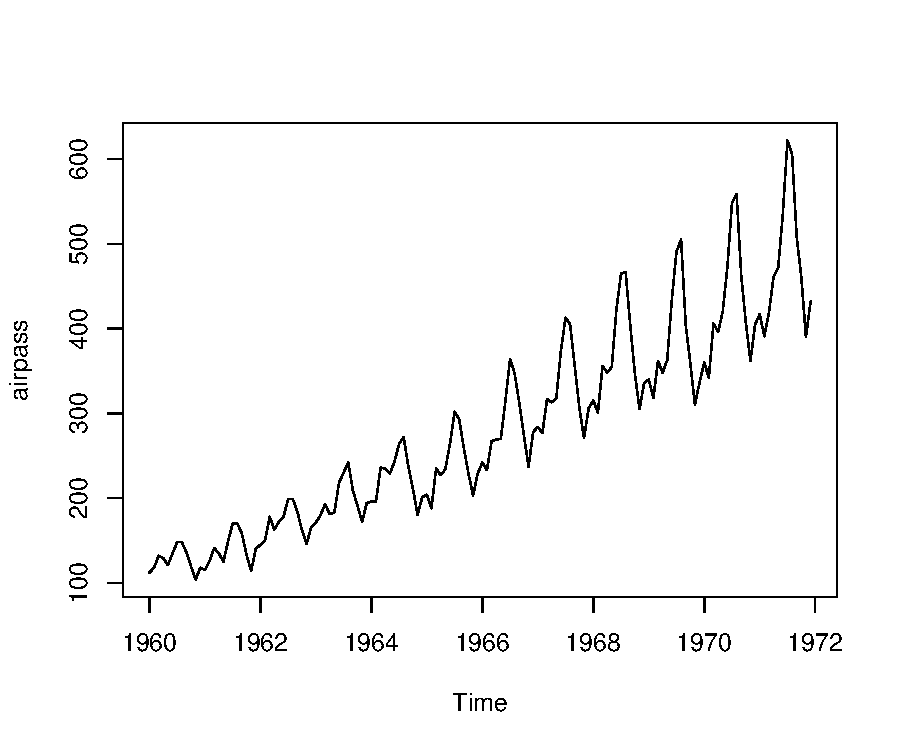
\includegraphics[width=0.47\linewidth]{images/airpass-plot}}
    \quad
    \subfigure[The logarithms of the series]{\label{ts.log}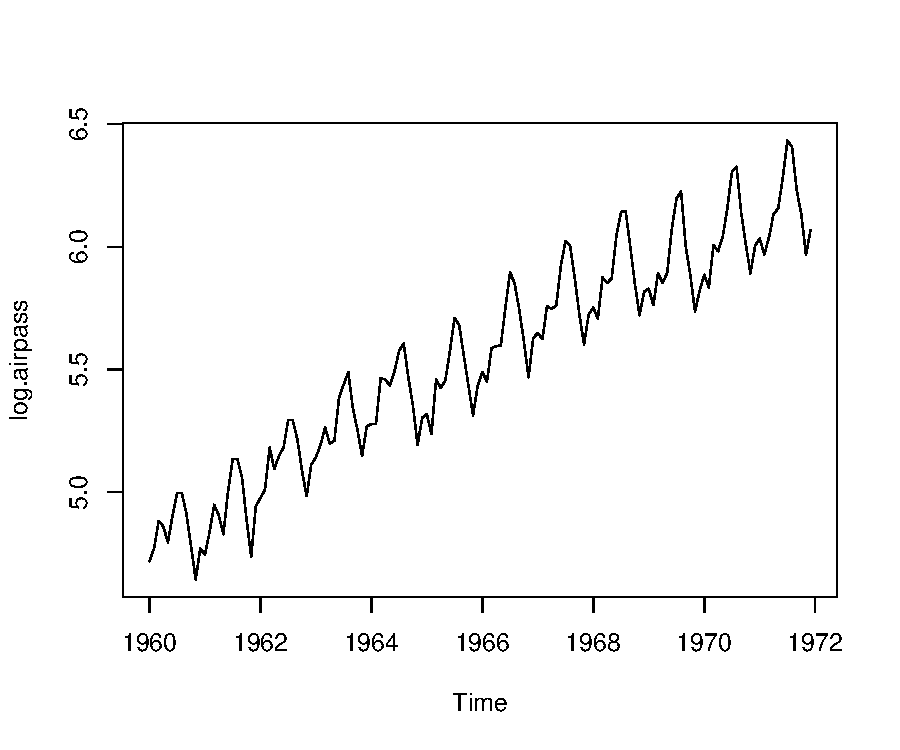
\includegraphics[width=0.47\linewidth]{images/log.airpass-plot}}
    \caption{The plot of the time series}
    \label{series}
\end{figure}

\vspace{4pt}
\textbf{Subproblem (b)}

As we can see from Figure \ref{diff-log}, after taking the first difference of the logged series, we can remove the linear trend of the logged series.
\begin{figure}[H]
    \centering
    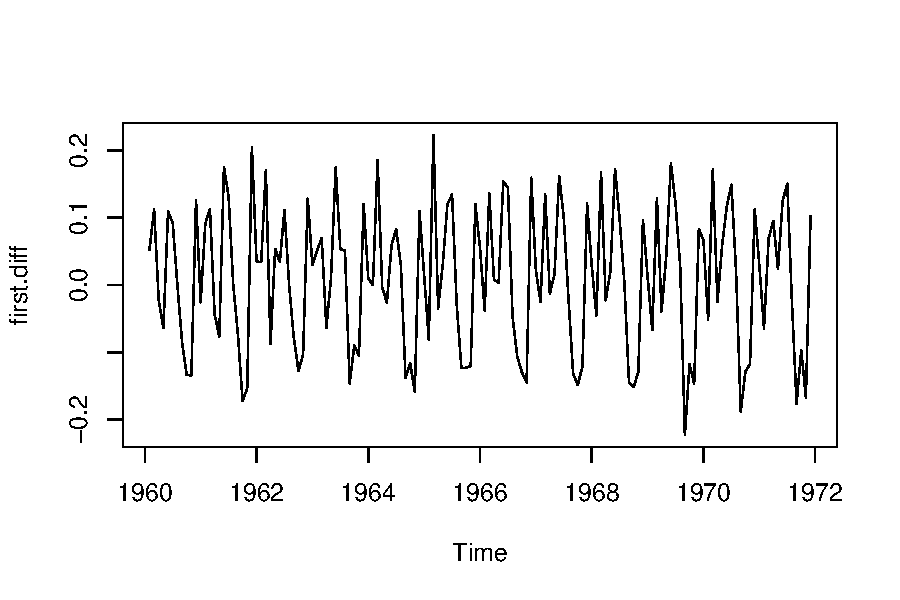
\includegraphics[width=0.65\linewidth]{images/diff1-log-series}
    \caption{The first difference of the logged series}
    \label{diff-log}
\end{figure}

\vspace{4pt}
\textbf{Subproblem (c)}

As we can see from Figure \ref{season-diff-log}, the seasonal difference of the first difference of the logged series seems not stationary, because the 
variance seems to vary as the trend increases.
\begin{figure}[H]
    \centering
    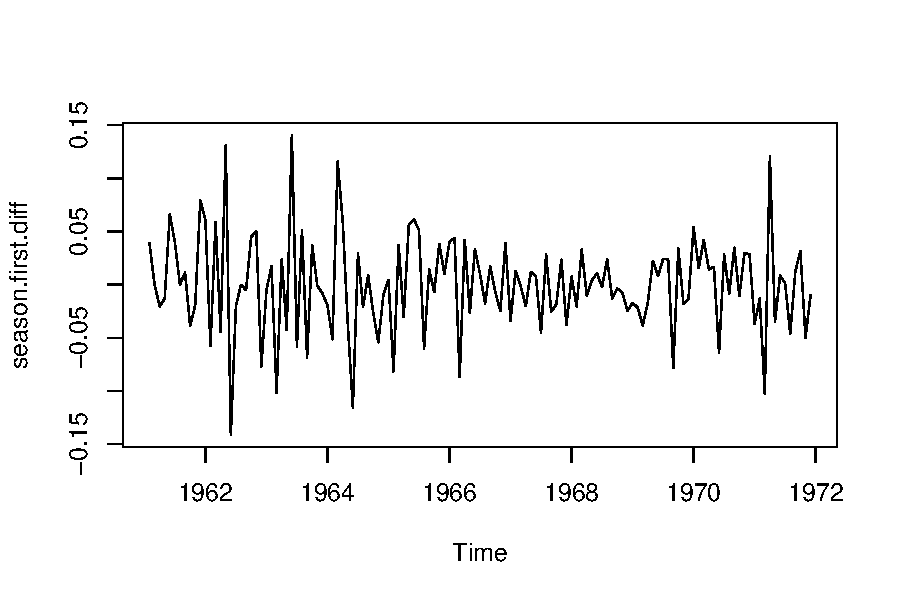
\includegraphics[width=0.65\linewidth]{images/season-diff-log-series}
    \caption{The seasonal difference of the first difference of the logged series}
    \label{season-diff-log}
\end{figure}

\vspace{4pt}
\textbf{Subproblem (d)}

As we can see from Figure \ref{acf-season-first-diff}, there is evident acf of the seasonal difference of the first difference of the logged series. 
\begin{figure}[H]
    \centering
    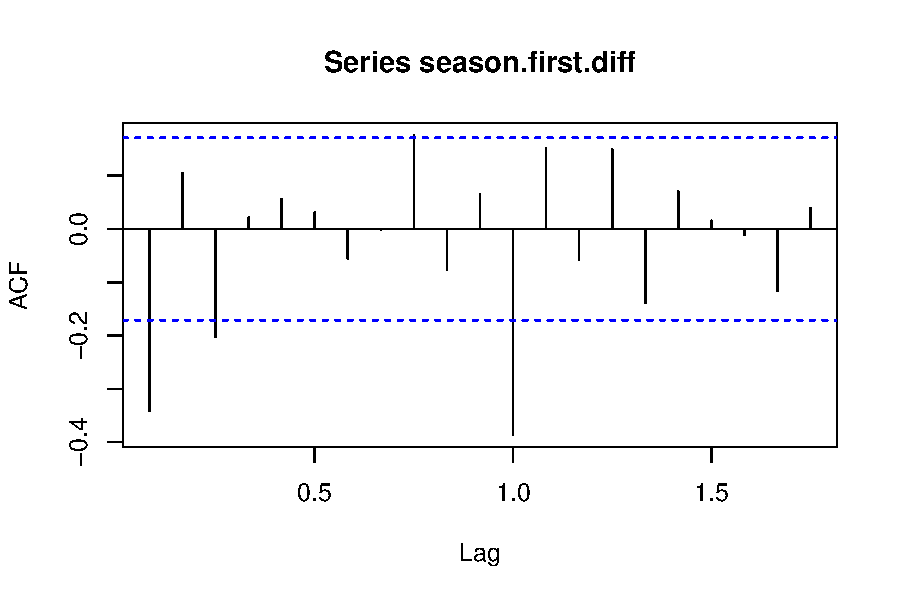
\includegraphics[width=0.65\linewidth]{images/acf-season-first-diff}
    \caption{The ACF of the seasonal difference of the first difference of the logged series}
    \label{acf-season-first-diff}
\end{figure}

\vspace{4pt}
\textbf{Subproblem (e)}

We use the following code to fit (ARIMA(0,1,1)(0,1,1)12) to the logged series. 
\begin{lstlisting}
log.airpass.arima = stats::arima(log.airpass, order=c(0,1,1), 
                    seasonal=list(order=c(0,1,1), period=12))
\end{lstlisting}
The fitted curve is showed as Figure \ref{log.airpass.arima.fit}. In this figure, the black line is the logged series, and the 
red dashed line is the fitted value by (ARIMA(0,1,1)(0,1,1)12).
\begin{figure}[H]
    \centering
    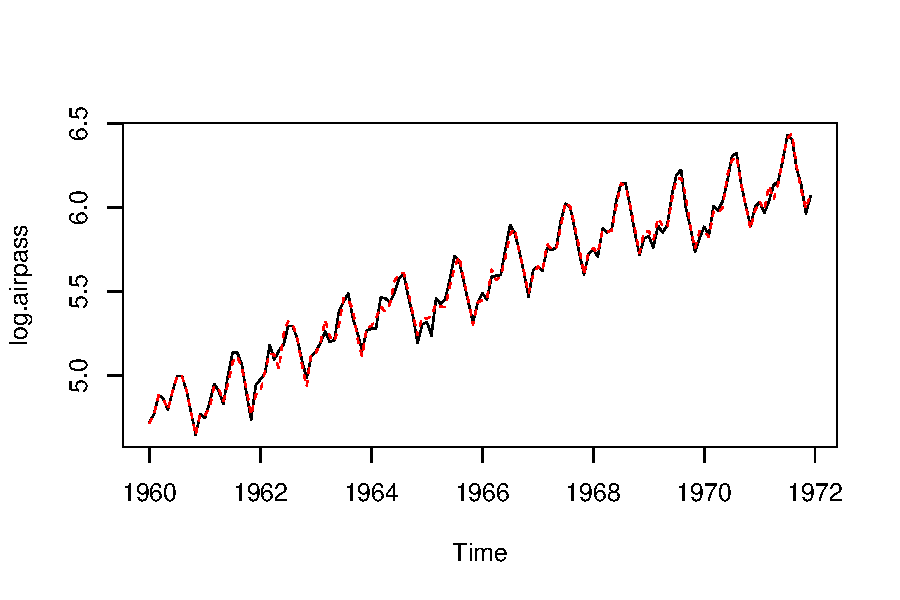
\includegraphics[width=0.65\linewidth]{images/log.airpass.arima.fit}
    \caption{The fitted figure of Seasonal ARIMA model}
    \label{log.airpass.arima.fit}
\end{figure}

\vspace{4pt}
\textbf{Subproblem (f)}

As we can see from Figure \ref{arima-check-res}, there is significant acf, so that the model is not very good. However, we can do the Ljung-Box test of the residuals to see if the residuals exhibit serial correlation, the result is as follow:
\begin{lstlisting}
        Box-Ljung test
data:  log.airpass.arima$residuals
X-squared = 8.8097, df = 9, p-value = 0.455
\end{lstlisting}
As we can see from the Ljung-Box test, the p-value equals 0.455, which is larger than 0.05, so that we should not reject the null hypothesis, which means 
the residuals does not exhibit serial correlation. Thus, we can believe that the Seasonal ARIMA model is suitable.

\begin{figure}[H]
    \centering
    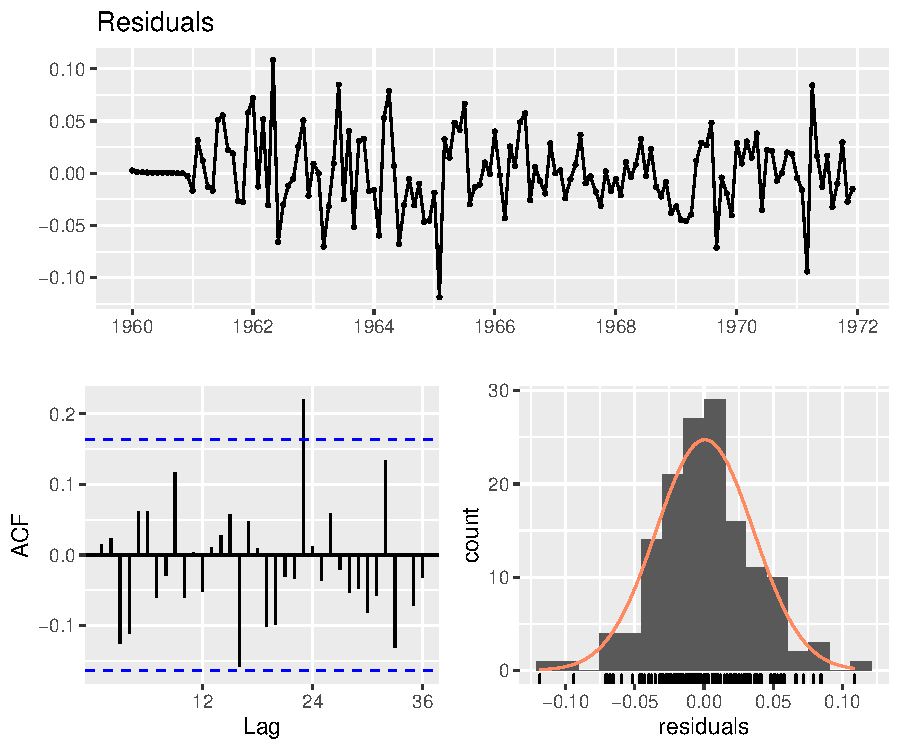
\includegraphics[width=0.6\linewidth]{images/arima-check-res}
    \caption{Check the residuals of Seasonal ARIMA}
    \label{arima-check-res}
\end{figure}

Then, we would like to check the normality of the residuals. We use Shapiro-Wilk normality test to test the normality. The result is as follow.
\begin{lstlisting}
Shapiro-Wilk normality test

data:  log.airpass.arima$residuals
W = 0.98637, p-value = 0.1674
\end{lstlisting}
As we can see from the result of Shapiro-Wilk normality test, p-value equals 0.1674, which is larger than 0.05, so we can conclude that the residuals is subject to normal distribution.

\vspace{4pt}
\textbf{Subproblem (g)}

The forecast for this series with a lead time of two years is as Figure \ref{log.airpass.arima.forecast}.
\begin{figure}[H]
    \centering
    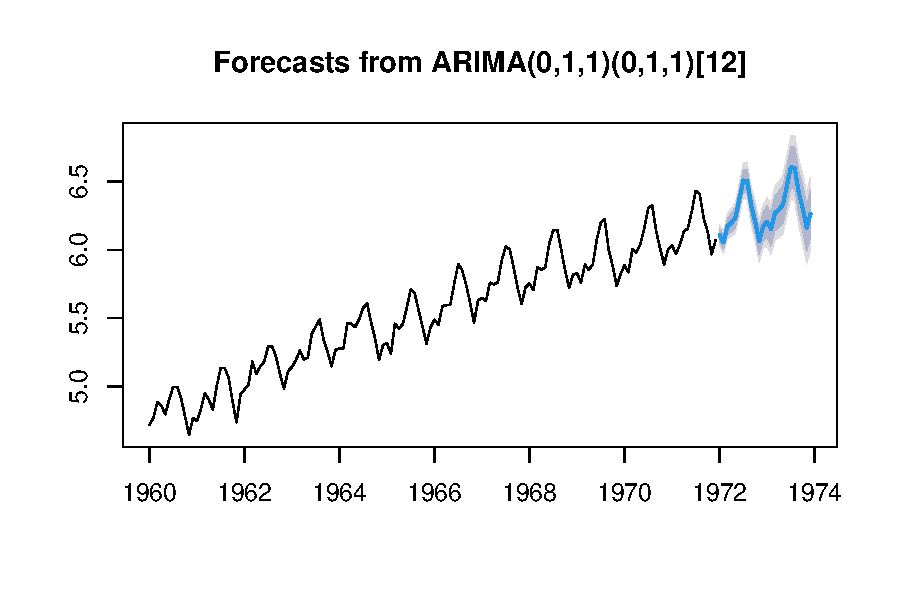
\includegraphics[width=0.6\linewidth]{images/log.airpass.arima.forecast}
    \vspace{-20pt}
    \caption{The forecast with Seasonal ARIMA model in two years}
    \label{log.airpass.arima.forecast}
\end{figure}
\end{homeworkProblem}

\begin{homeworkProblem}
Consider the model $Y_{t}=e_{t-1}-e_{t-2}+0.5 e_{t-3}$.
\begin{enumerate}[(a)]
    \item Find the autocovariance function for this process.
    \item Argue this is just an $MA$ process in disguise. What is that process?
\end{enumerate}

\vspace{4pt}
\textbf{\large{Solution}}

\vspace{4pt}
\textbf{Subproblem (a)}

We suppose $e_t\sim IWN\left(0,\sigma^2\right)$. Then, we can derive the autocovariance function as follow
\begin{equation}
    \begin{split}
        \gamma_k &= \operatorname{Cov}\left(Y_t, Y_{t+k}\right)\\
        &=\operatorname{Cov}\left(e_{t-1}-e_{t-2}+0.5e_{t-3}, e_{t+k-1}-e_{t+k-2}+0.5e_{t+k-3}\right)\\
        \Longrightarrow\gamma_k &= 
        \begin{cases}
            2.25\sigma^2 &\left(k=0\right)\\
            -1.5\sigma^2&\left(k=1\right)\\
            0.5\sigma^2&\left(k=2\right)\\
            0&\left(k>2\right)
        \end{cases}
    \end{split}
\end{equation}

\vspace{4pt}
\textbf{Subproblem (b)}

Actually, this is just an MA(2) process in disguise. This is because the error term $e_t$ is a random variable and actually the same thing 
in different time. Thus, we can treat the original series as follow
\begin{equation}
    Y_{t}=e_{t}-e_{t-1}+0.5 e_{t-2}
\end{equation}
Thus, this is a MA(2) process with parameters $\phi_2\left(\boldsymbol{B}\right) =1-\boldsymbol{B}+0.5\boldsymbol{B}^2$.
\end{homeworkProblem}

\begin{homeworkProblem}
Identify as specific \textit{ARIMA} models, that is, what are $p, d$, and $q$ and what are the values of the parameters- the $\phi$ 's and $\theta$ 's? Note: For the model to be an $A R I M A$ model, the $A R M A$ part needs to be stationary. You may need to determine how many differences to take.
\begin{enumerate}[(a)]
    \item $Y_{t}=Y_{t-1}-0.25 Y_{t-2}+e_{t}-0.1 e_{t-1}$
    \item $Y_{t}=2 Y_{t-1}-Y_{t-2}+e_{t}$
    \item $Y_{t}=0.5 Y_{t-1}-0.5 Y_{t-2}+e_{t}-0.5 e_{t-1}+0.25 e_{t-2}$
\end{enumerate}

\vspace{4pt}
\textbf{\large{Solution}}

\vspace{4pt}
\textbf{Subproblem (a)}

The characteristic equation of the AR process is 
\begin{equation}
    \theta_2\left(\boldsymbol{B}\right)=1-\boldsymbol{B}+0.25\boldsymbol{B}^2=0
\end{equation}
Thus, we can derive the roots are $\boldsymbol{B}_1=\boldsymbol{B}_2=2$. Thus, the process is stationary, so we can derive $p,d,q$ and the 
parameters of the $\phi$ 's and $\theta$ 's as follow.
\begin{equation}
    \begin{split}
        &p = 2\\
        &q =1\\
        &d =0\\
        &\theta_2\left(\boldsymbol{B}\right) = 1-\boldsymbol{B}+0.25\boldsymbol{B}^2\\
        &\phi_1\left(\boldsymbol{B}\right) = 1-0.1\boldsymbol{B}
    \end{split}
\end{equation}

\vspace{4pt}
\textbf{Subproblem (b)}

The characteristic equation of the AR process is 
\begin{equation}
    \theta_2\left(\boldsymbol{B}\right)=1-2\boldsymbol{B}+\boldsymbol{B}^2=0
\end{equation}
Thus, we can derive the roots are $\boldsymbol{B}_1=\boldsymbol{B}_2=1$. Thus, the process is not stationary. 
Then can describe the process as follow
\begin{equation}
    \begin{split}
        &\left(1-2\boldsymbol{B}+\boldsymbol{B}^2\right)Y_t= e_t\\
        \Longrightarrow \quad  &\left(1-\boldsymbol{B}\right)^2Y_t=e_t
        \end{split}
\end{equation}
Thus, the second order difference of $Y_t$ is stationary, so we can derive $p,d,q$ and the 
parameters of the $\phi$ 's and $\theta$ 's as follow.
\begin{equation}
    \begin{split}
        &p = 0\\
        &q =0\\
        &d =2\\
        &\theta_0\left(\boldsymbol{B}\right) = 1\\
        &\phi_0\left(\boldsymbol{B}\right) = 1
    \end{split}
\end{equation}

\vspace{4pt}
\textbf{Subproblem (c)}

The characteristic equation of the AR process is 
\begin{equation}
    \theta_2\left(\boldsymbol{B}\right)=1-0.5\boldsymbol{B}+0.5\boldsymbol{B}^2=0
\end{equation}
Thus, we can derive the roots are $\boldsymbol{B}_1=\frac{1}{2}+\frac{\sqrt{7}}{2}i,\boldsymbol{B}_2=\frac{1}{2}-\frac{\sqrt{7}}{2}i$. We know the absolute value of $\boldsymbol{B}_1$ and $\boldsymbol{B}_2$ are $\sqrt{2}$, which is larger than 1. Thus, the process is stationary, so we can derive $p,d,q$ and the 
parameters of the $\phi$ 's and $\theta$ 's as follow.
\begin{equation}
    \begin{split}
        &p = 2\\
        &q =2\\
        &d =0\\
        &\theta_2\left(\boldsymbol{B}\right) = 1-0.5\boldsymbol{B}+0.5\boldsymbol{B}^2\\
        &\phi_2\left(\boldsymbol{B}\right) = 1-0.5\boldsymbol{B}+0.25\boldsymbol{B}^2
    \end{split}
\end{equation}
\end{homeworkProblem}

\begin{homeworkProblem}
Describe the important characteristics of the autocorrelation function for the following models: (a) $M A(1)$, (b) $M A(2)$, (c) $A R(1)$, and $($d) $A R M A(1,1)$. Simulate a series for each of them with $T=10000$, and show the ACF plots.

\vspace{4pt}
\textbf{\large{Solution}}

\vspace{4pt}
\textbf{Subproblem (a)}

For the $MA\left(1\right)$ process, we have 
\begin{equation}
    Y_t = e_t + \beta e_{t-1}
\end{equation}
Then, we can derive the autocorrelation function as follow
\begin{equation}
    \begin{split}
        \rho_k = 
        \begin{cases}
            1&\left(k=0\right)\\
            \frac{\beta}{1+\beta^2}&\left(k=1\right)\\
            0&\left(k>1\right)
        \end{cases}
    \end{split}
\end{equation}
Then, we simulate $MA(1)$ with $\beta=1$, and show the ACF plot as Figure \ref{ma1}.
\begin{figure}[H]
    \centering
    \subfigure[The simulated MA(1) series]{\label{}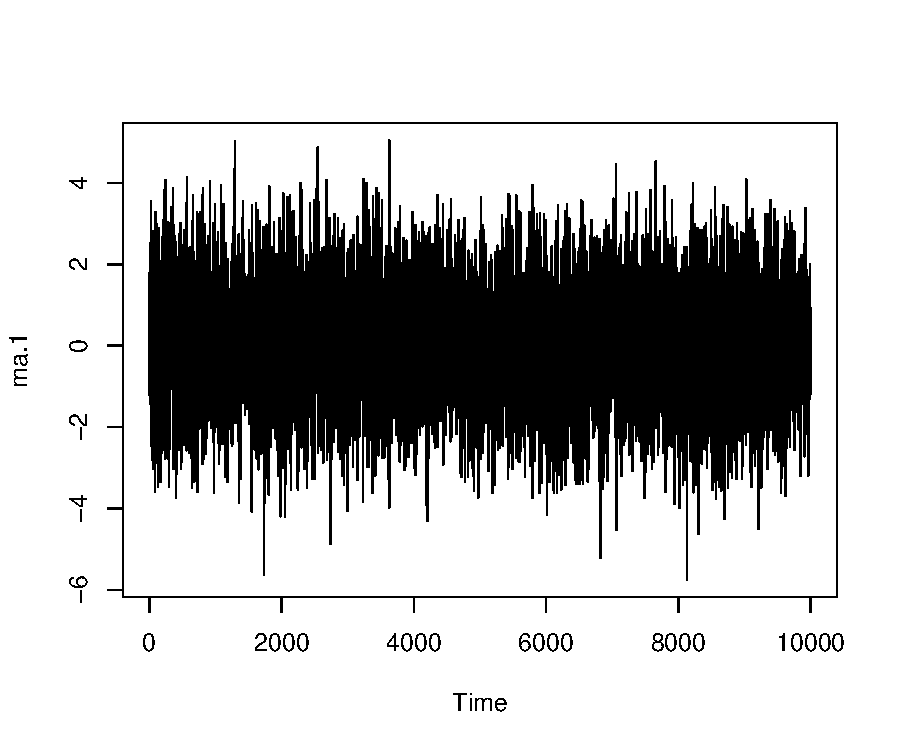
\includegraphics[width=0.47\linewidth]{images/ma1}}
    \quad
    \subfigure[The acf of simulated MA(1) series]{\label{}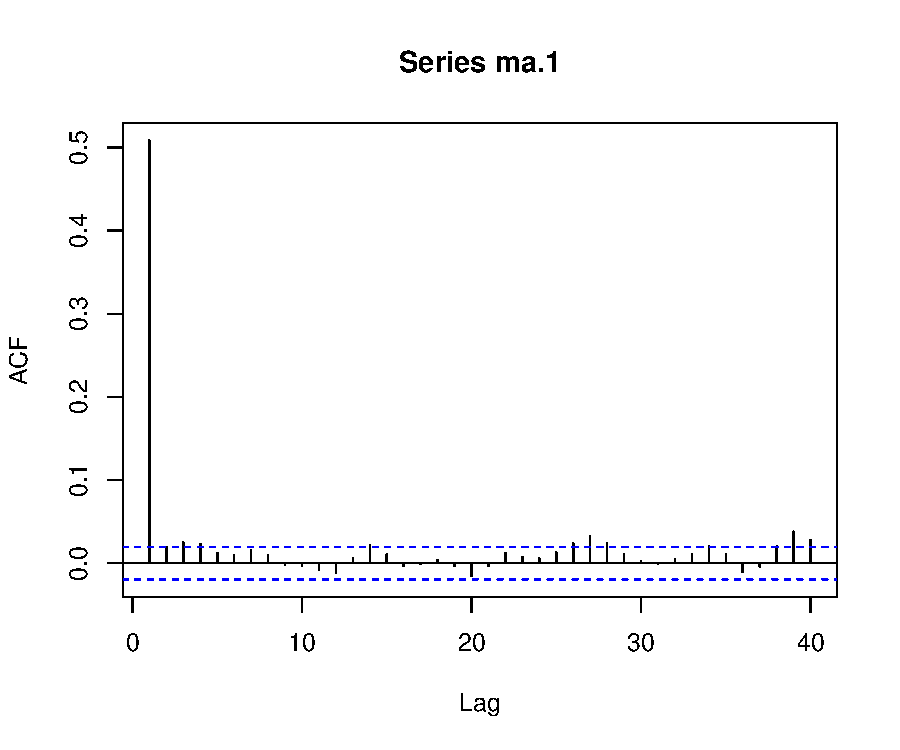
\includegraphics[width=0.47\linewidth]{images/ma1-acf}}
    \caption{The plot of simulated MA(1) process}
    \label{ma1}
\end{figure}

\vspace{4pt}
\textbf{Subproblem (b)}

For the $MA\left(2\right)$ process, we have  
\begin{equation}
    Y_t = e_t + \beta_1 e_{t-1} + \beta_2 e_{t-2}
\end{equation}
Then, we can derive the autocorrelation function as follow
\begin{equation}
    \begin{split}
        \rho_k = 
        \begin{cases}
            1&\left(k=0\right)\\
            \frac{\beta_1+\beta_1\beta_2}{1+\beta_1^2+\beta_2^2}&\left(k=1\right)\\
            \frac{\beta_2}{1+\beta_1^2+\beta_2^2}&\left(k=2\right)\\
            0&\left(k>2\right)
        \end{cases}
    \end{split}
\end{equation}
Then, we simulate $MA(1)$ with $\beta_1=1, \beta_2=0.5$, and show the ACF plot as Figure \ref{ma2}.
\begin{figure}[H]
    \centering
    \subfigure[The simulated MA(2) series]{\label{}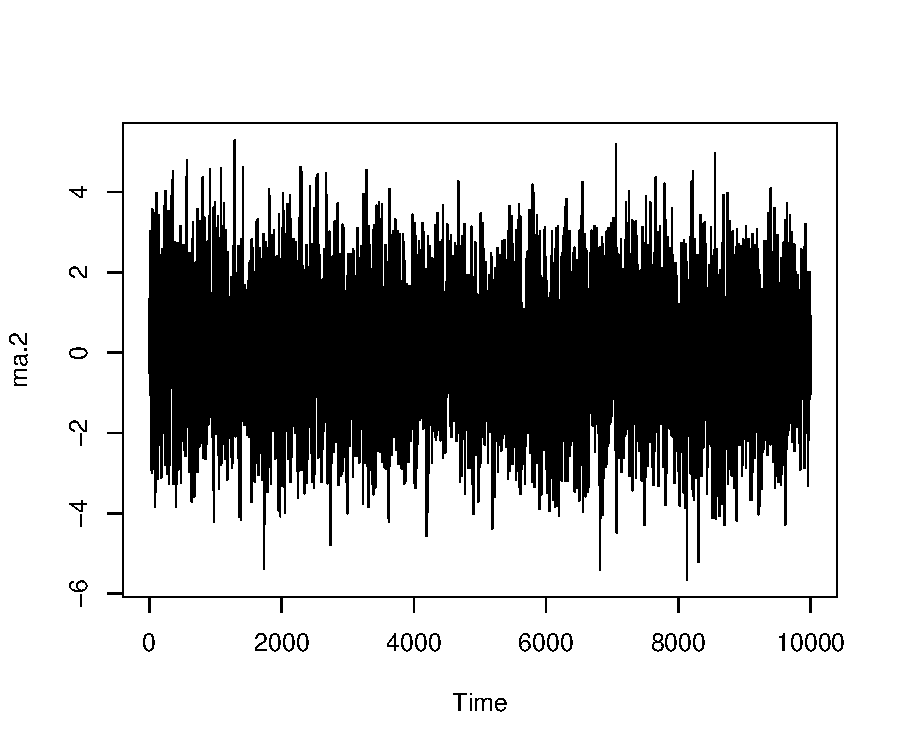
\includegraphics[width=0.47\linewidth]{images/ma2}}
    \quad
    \subfigure[The acf of simulated MA(2) series]{\label{}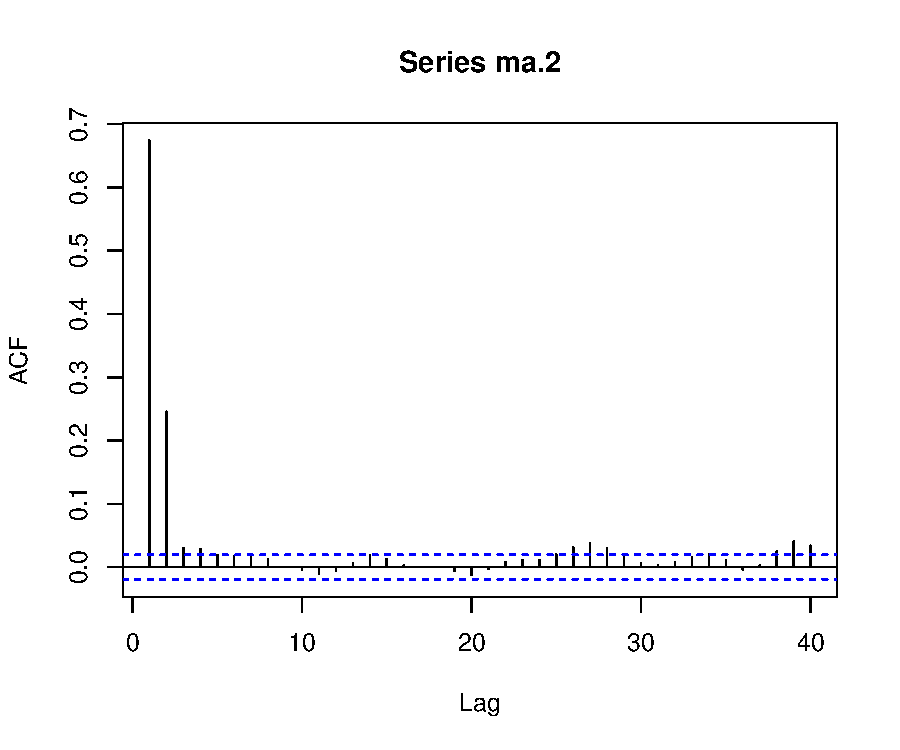
\includegraphics[width=0.47\linewidth]{images/ma2-acf}}
    \caption{The plot of simulated MA(2) process}
    \label{ma2}
\end{figure}

\vspace{4pt}
\textbf{Subproblem (c)}

For the $AR\left(1\right)$ process, we have  
\begin{equation}
    Y_t = \alpha Y_{t-1}+e_t
\end{equation}
Then, we can derive the autocorrelation function as follow
\begin{equation}
    \rho_k = \alpha^k
\end{equation}
Then, we simulate $AR(1)$ with $\alpha=0.5$, and show the ACF plot as Figure \ref{ar1}.
\begin{figure}[H]
    \centering
    \subfigure[The simulated AR(1) series]{\label{}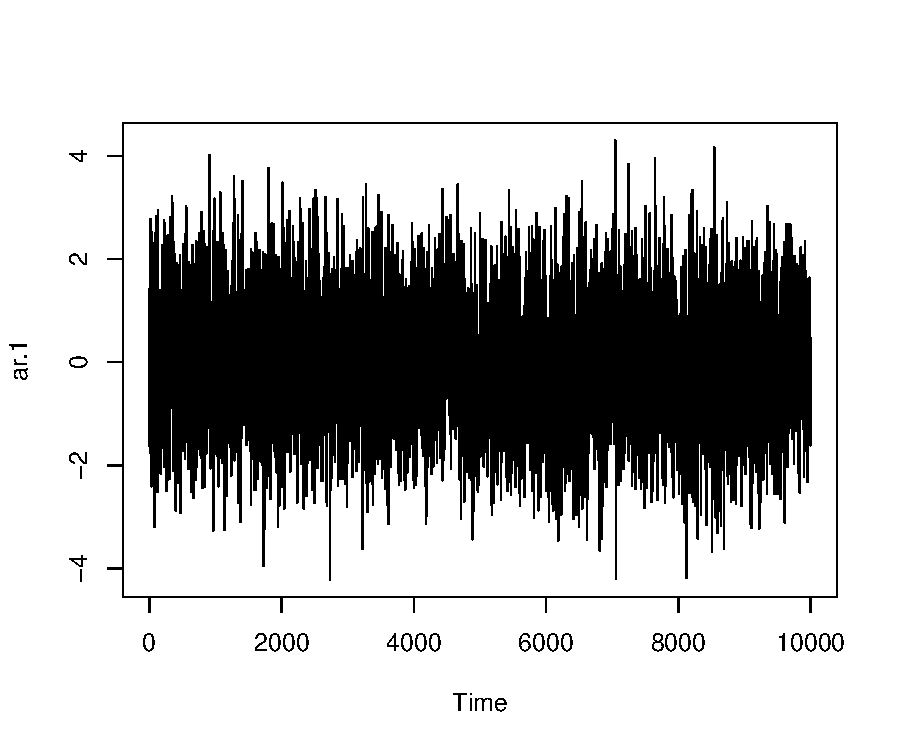
\includegraphics[width=0.47\linewidth]{images/ar1}}
    \quad
    \subfigure[The acf of simulated AR(1) series]{\label{}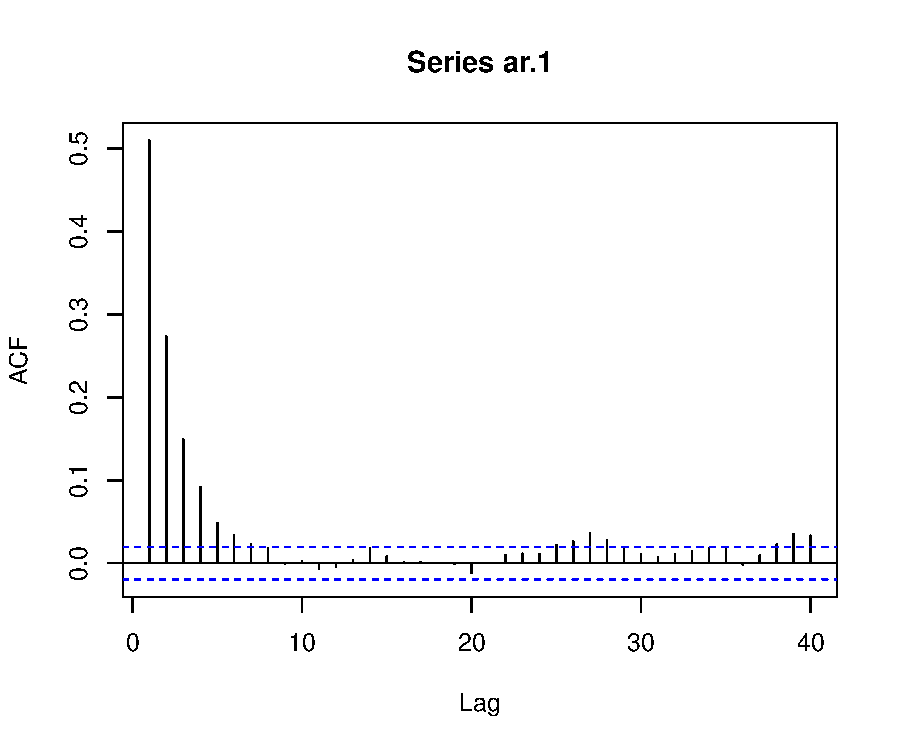
\includegraphics[width=0.47\linewidth]{images/ar1-acf}}
    \caption{The plot of simulated AR(1) process}
    \label{ar1}
\end{figure}

\vspace{4pt}
\textbf{Subproblem (d)}

For the $ARMA\left(1,1\right)$ process, we have  
\begin{equation}
    Y_t = \alpha Y_{t-1}+e_t+\beta e_{t-1}
\end{equation}
Then, we can derive the autocorrelation function as follow
\begin{equation}
    \rho_k = 
    \begin{cases}
        1&\left(k=0\right)\\
        \frac{\alpha^{k-1}\left(\alpha+\beta\right)\left(1+\alpha\beta\right)}{1+2\alpha\beta+\beta^2}&\left(k\geq1\right)
    \end{cases}
\end{equation}
Then, we simulate $ARMA(1,1)$ with $\alpha=0.7, \beta=0.5$, and show the ACF plot as Figure \ref{arma11}.
\begin{figure}[H]
    \centering
    \subfigure[The simulated ARMA(1,1) series]{\label{}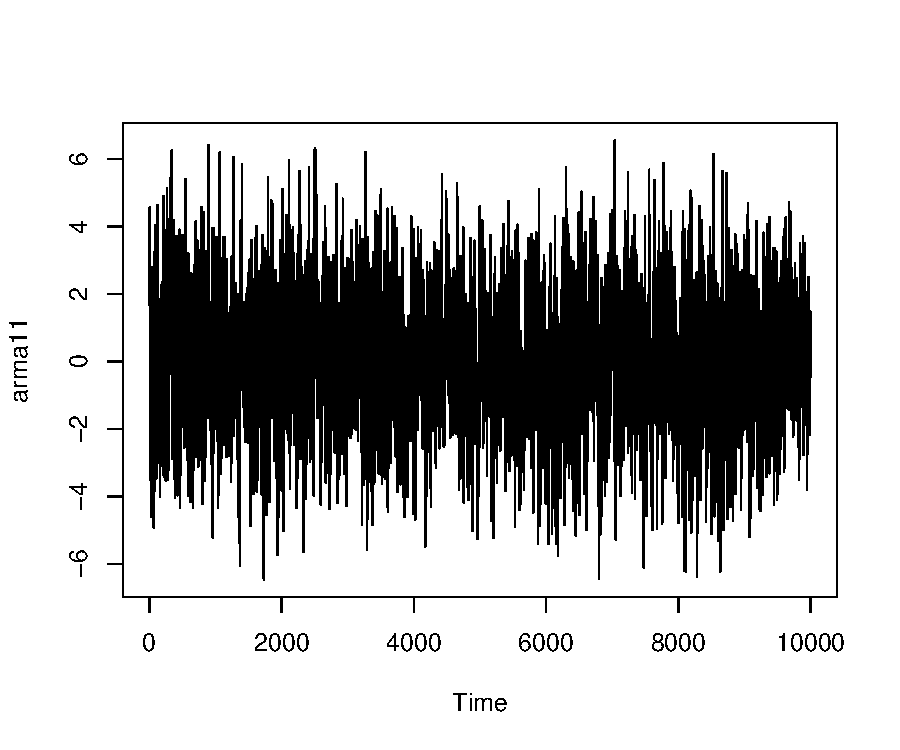
\includegraphics[width=0.47\linewidth]{images/arma11}}
    \quad
    \subfigure[The acf of simulated ARMA(1,1) series]{\label{}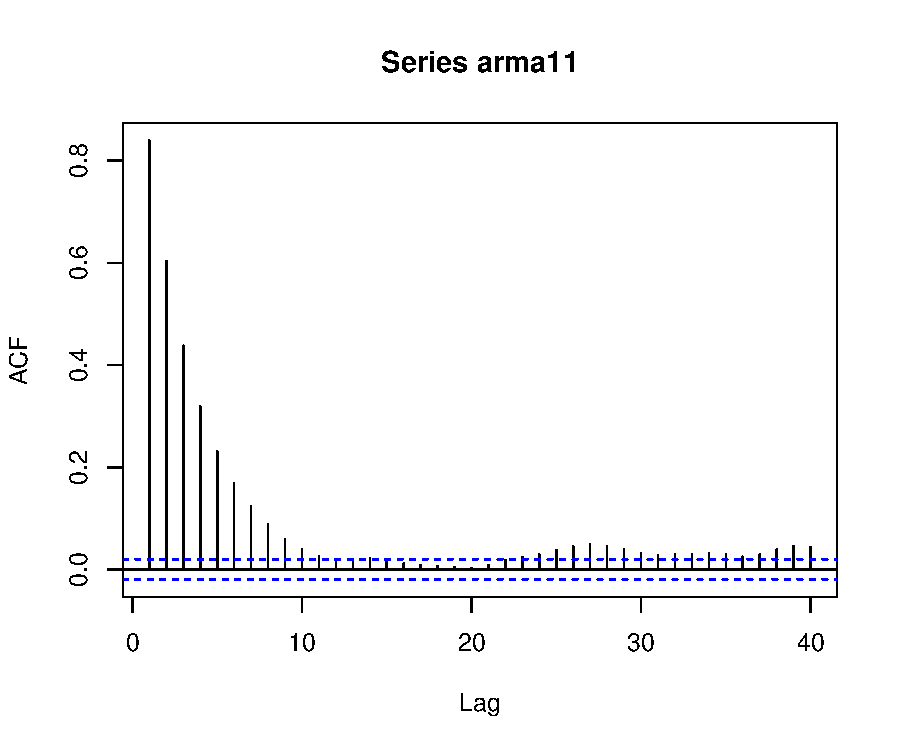
\includegraphics[width=0.47\linewidth]{images/arma11-acf}}
    \caption{The plot of simulated ARMA(1,1) process}
    \label{arma11}
\end{figure}
\end{homeworkProblem}

\begin{homeworkProblem}
The daily returns of Google stock from August 14, 2004 to September 13, 2006 are stored in data(google) in the package $T S A$.
\begin{enumerate}[(a)]
    \item Display the time sequence plot for the return data and show that the data are essentially uncorrelated over time. Is there changes in variance over time?
    \item Fit $G A R C H(1,1)$ model for the Google daily return data. Draw and comment on the time sequence plot of the estimated conditional variances. Does the model appear to have addressed the conditional heteroskedasticity?
\end{enumerate} 

\vspace{4pt}
\textbf{\large{Solution}}

\vspace{4pt}
\textbf{Subproblem (a)}

We plot the google stock daily return time series as Figure \ref{google-ts}, and the acf of google stock daily return time series as 
Figure \ref{google-acf}. As we can see, there is no evident autocorrelation over time. Thus, the data are essentially uncorrelated over time.

\vspace{4pt}
As we can see from Figure \ref{google-ts}, the variance seems not constant over time. Then, we can plot the correlogram of the squared values to detect the volatility as Figure \ref{google2}. 
As we can see, the variance is correlated in time, since the series exhibits volatility which can be derived from Figure \ref{google_squared_acf}.
\begin{figure}[H]
    \centering
    \subfigure[The time series]{\label{google-ts}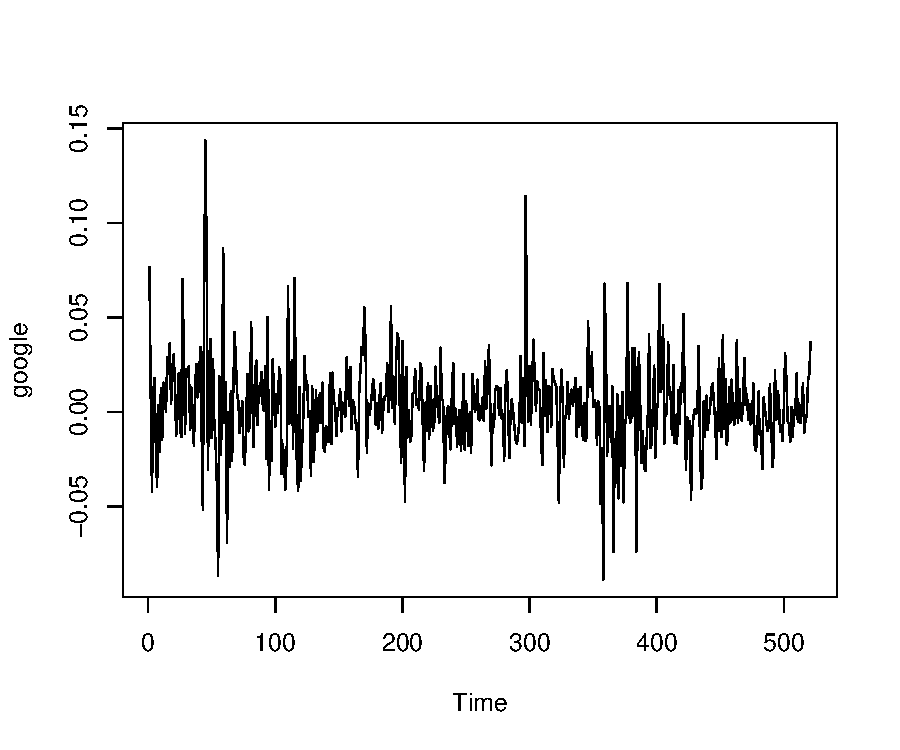
\includegraphics[width=0.47\linewidth]{images/google}}
    \quad
    \subfigure[The acf of the time series]{\label{google-acf}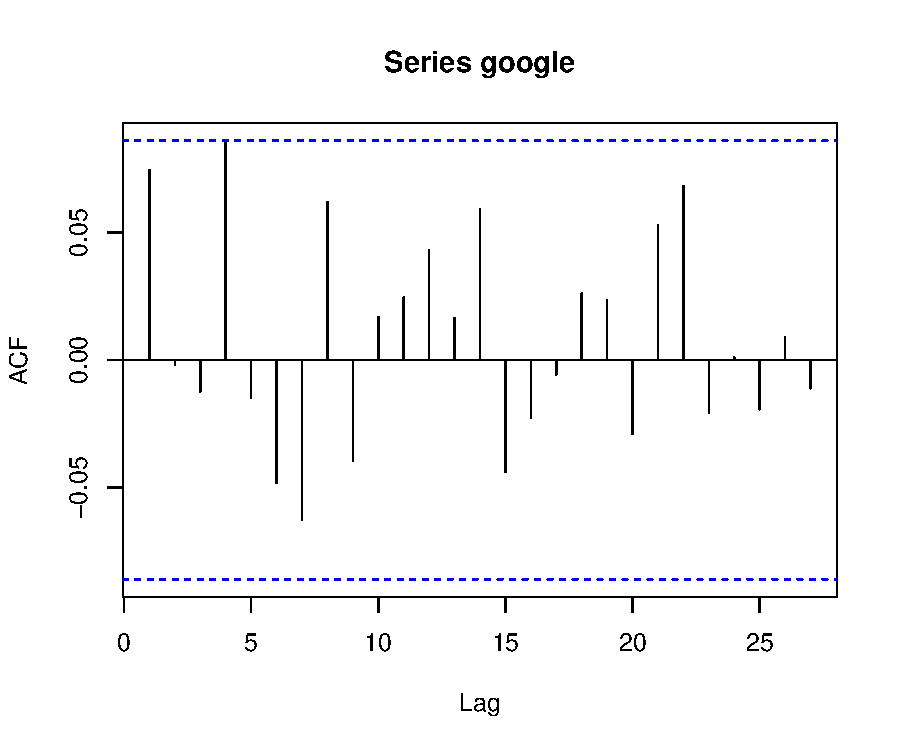
\includegraphics[width=0.47\linewidth]{images/google-acf}}
    \caption{The google stock daily return time series}
    \label{google}
\end{figure}

\begin{figure}[H]
    \centering
    \subfigure[The squared time series]{\label{}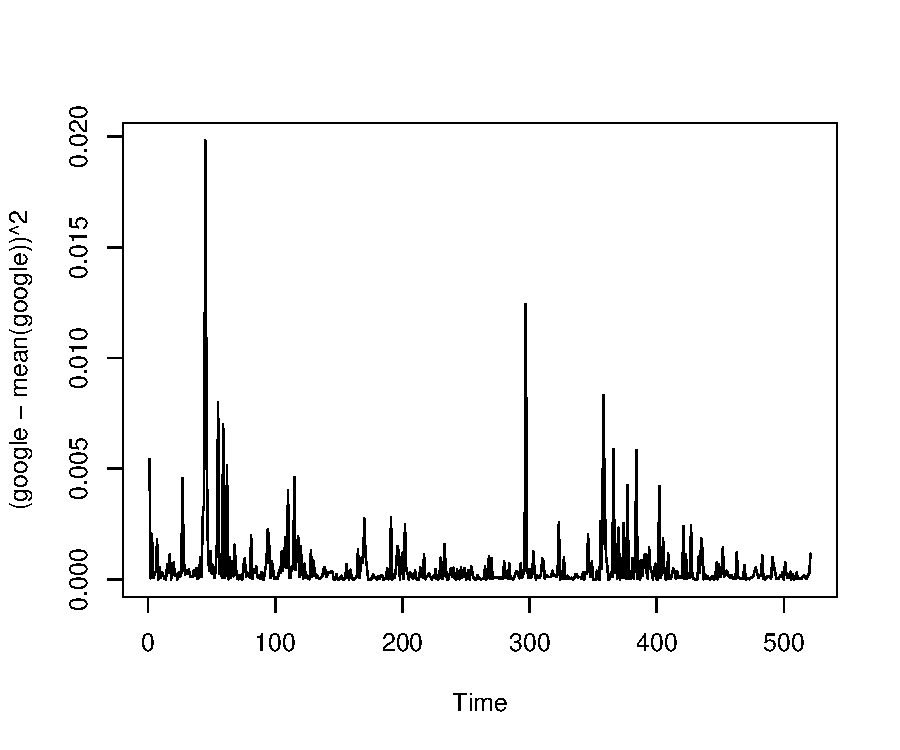
\includegraphics[width=0.47\linewidth]{images/google-2}}
    \quad
    \subfigure[The acf of the squared time series]{\label{google_squared_acf}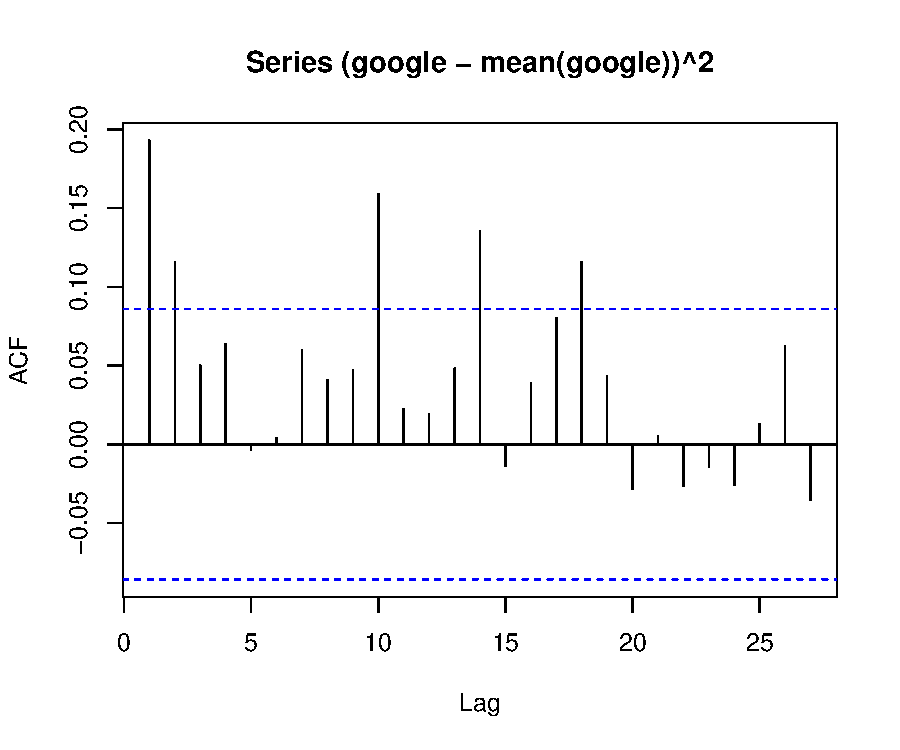
\includegraphics[width=0.47\linewidth]{images/google-2-acf}}
    \caption{The squared value of google stock daily return time series}
    \label{google2}
\end{figure}

\vspace{4pt}
\textbf{Subproblem (b)}

We fit the google daily return data with GARCH(1,1) model, the series with fitteds standard deviation is as Figure \ref{google-garch-fit}. 
And the time sequence plot of the estimated conditional variance is as Figure \ref{google-garch-var}. Then, we would like to check if the model 
have addressed the conditional heteroskedasticity. As we know, if all estimated conditional variance captures the conditional variance, the residuals will be white 
noise with mean 0 and variance 1. 

\vspace{4pt}

Thus, we would like to check the residuals. The test result is as follow and the test figures are as Figure \ref{google-res}. 
\begin{lstlisting}
Diagnostic Tests:
	Jarque Bera Test

data:  Residuals
X-squared = 223.48, df = 2, p-value < 2.2e-16
	Box-Ljung test

data:  Squared.Residuals
X-squared = 0.0004683, df = 1, p-value = 0.9827
\end{lstlisting}
As we can see from the Jarque Bera Test result, the $p$-value $<2.2e^{-16}$, which means the distribution of residuals is not normal. On the other hand, as we can see 
from the Box-Ljung test result, the $p$-value equals 0.9827, which means there is no serial autocorrelation in residuals. With the ACF figure of residuals in
Figure \ref{google-res}, we ca derive that the residuals can be 
treated as white noise, which means the GARCH(1,1) model has addressed the conditional heteroskedasticity, although the distribution of residuals is not normal.
\begin{figure}[H]
    \centering
    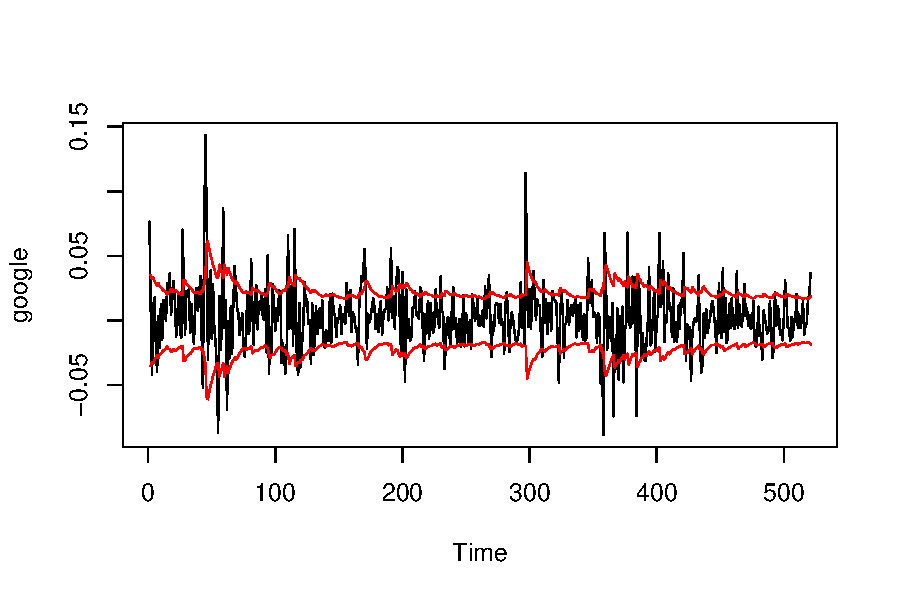
\includegraphics[width=0.5\linewidth]{images/google-garch-fit}
    \caption{The google daily return data with GARCH(1,1) model}
    \label{google-garch-fit}
\end{figure}
\begin{figure}[H]
    \centering
    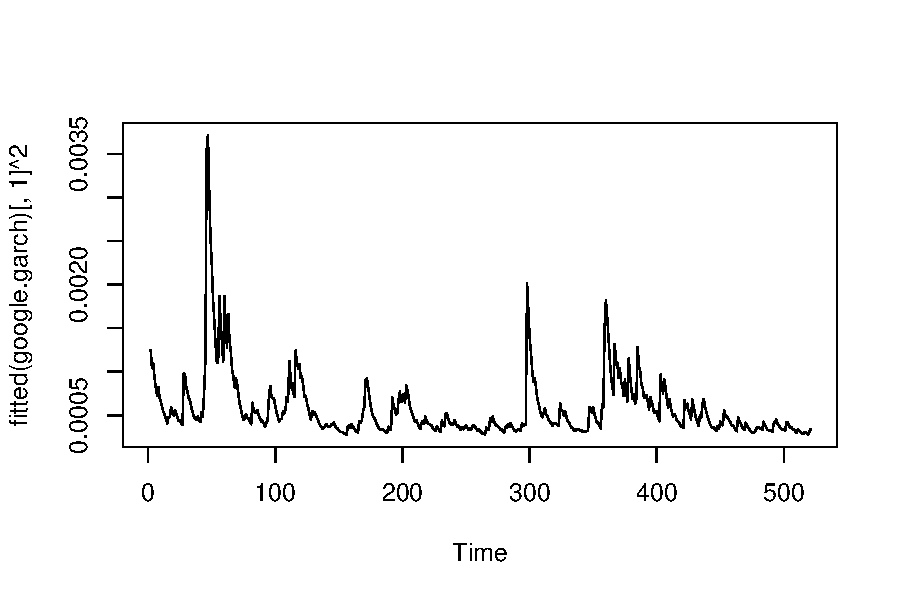
\includegraphics[width=0.5\linewidth]{images/google-garch-var}
    \caption{The time sequence plot of the estimated conditional variance}
    \label{google-garch-var}
\end{figure}
\begin{figure}[H]
    \centering
    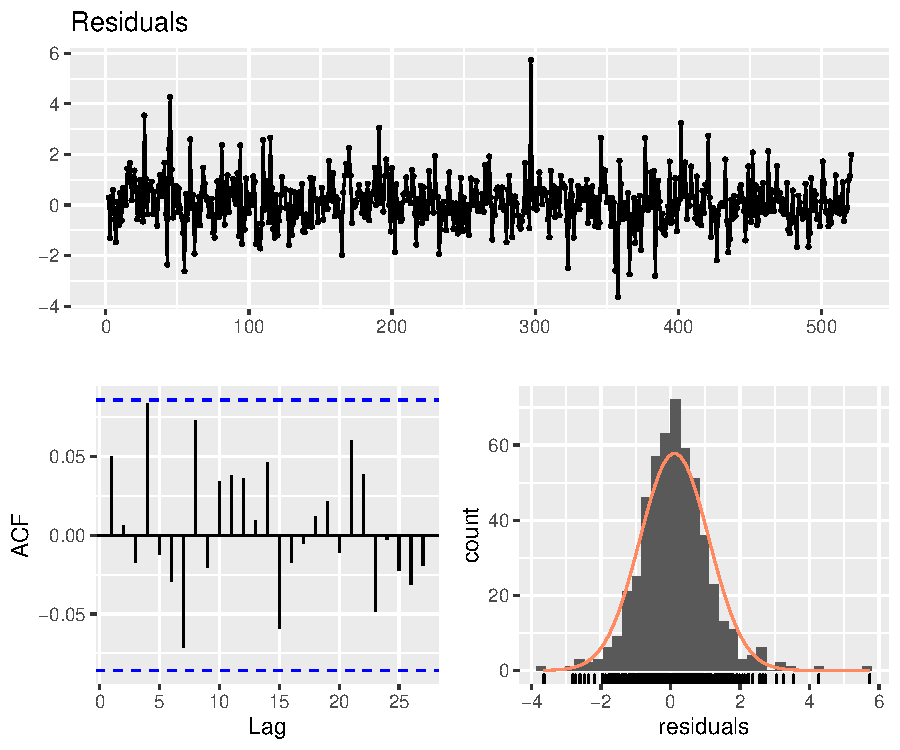
\includegraphics[width=0.6\linewidth]{images/google-res}
    \caption{The check of residuals}
    \label{google-res}
\end{figure}

\end{homeworkProblem}




\begin{homeworkProblem}
Consider the $A R(1)$ model
$$
Y_{t}=\phi Y_{t-1}+e_{t}
$$
The theoretical spectral density is
$$
S(f)=\frac{\sigma_{e}^{2}}{1+\phi^{2}-2 \phi \cos (2 \pi f)}
$$
\begin{enumerate}[(a)]
    \item Show that when $\phi>0$ the spectral density for an $A R(1)$ process is a decreasing function of frequency, while for $\phi<0$ the spectral density increases.
    \item Graph the theoretical spectral density for an $A R(1)$ time series with $\phi=0.7$. Interpret the implications of the shape of the spectrum on the possible plots of the time series values.
    \item Graph the theoretical spectral density for an $A R(1)$ time series with $\phi=-0.4$. Interpret the implications of the shape of the spectrum on the possible plots of the time series values.    
\end{enumerate}

\vspace{4pt}
\textbf{\large{Solution}}

\vspace{4pt}
\textbf{Subproblem (a)}

We can derive the derivative function of $S(f)$ as follow
\begin{equation}
    \begin{split}
        S^{\prime}(f) = \frac{-4\pi\phi\sigma_{e}^{2}\sin\left(2\pi f\right)}{\left[1+\phi^{2}-2 \phi \cos (2 \pi f)\right]^2}
    \end{split}
\end{equation} 
We know that when $f\in [0,\frac{1}{2}], \sin\left(2\pi f\right)\geq 0$. Thus, we have
\begin{equation}
    \begin{split}
        \begin{cases}
            S^{\prime}(f)\leq 0 &\left(\phi >0\right)\\
            S^{\prime}(f)\geq 0 &\left(\phi <0\right)\\
        \end{cases}
    \end{split}
\end{equation}
Thus, we can derive when $\phi>0$ the spectral density for an $A R(1)$ process is a decreasing function of frequency, while for $\phi<0$ the spectral density increases.

\vspace{4pt}
\textbf{Subproblem (b)}

We plot the simulated $AR(1)$ time series with $\phi=0.7$ as Figure \ref{ar1-q6}. As we can see 
from Figure \ref{ar1-q6}, because $\phi=0.7$ is larger than 0, so there is no very strong variation in the time series. And we can see that 
the ACF is positive mostly.

\vspace{4pt}
We graph the theoretical spectral density for an $AR(1)$ time series with $\phi=0.7$ as Figure \ref{ar1-spec}. 
As we can see from Figure \ref{ar1-spec}, the spectral density decreases rapidly at the beginning and then decreases slowly later, which agreed with the conclusion derived in subproblem (a). 
Besides, the density is much stonger for lower frequencies than for high frequencies, this is because the time series's variation is 
not very strong, which means the process tends to change slowly from one time instance to the next.
\begin{figure}[H]
    \centering
    \subfigure[The AR(1) time series]{\label{}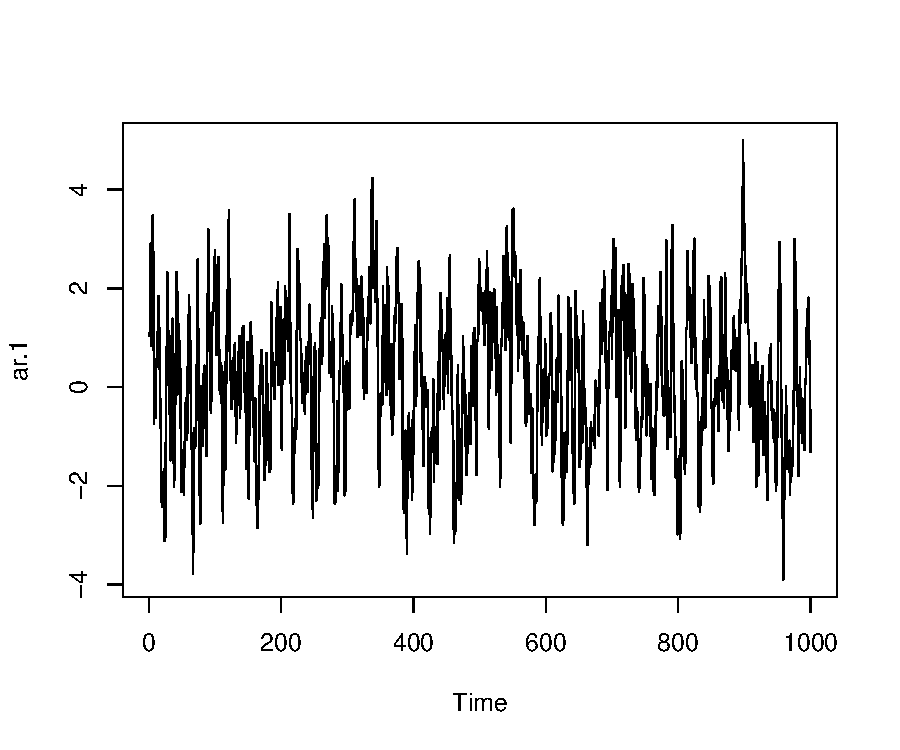
\includegraphics[width=0.47\linewidth]{images/ar1-q6}}
    \quad
    \subfigure[The acf of AR(1) time series]{\label{}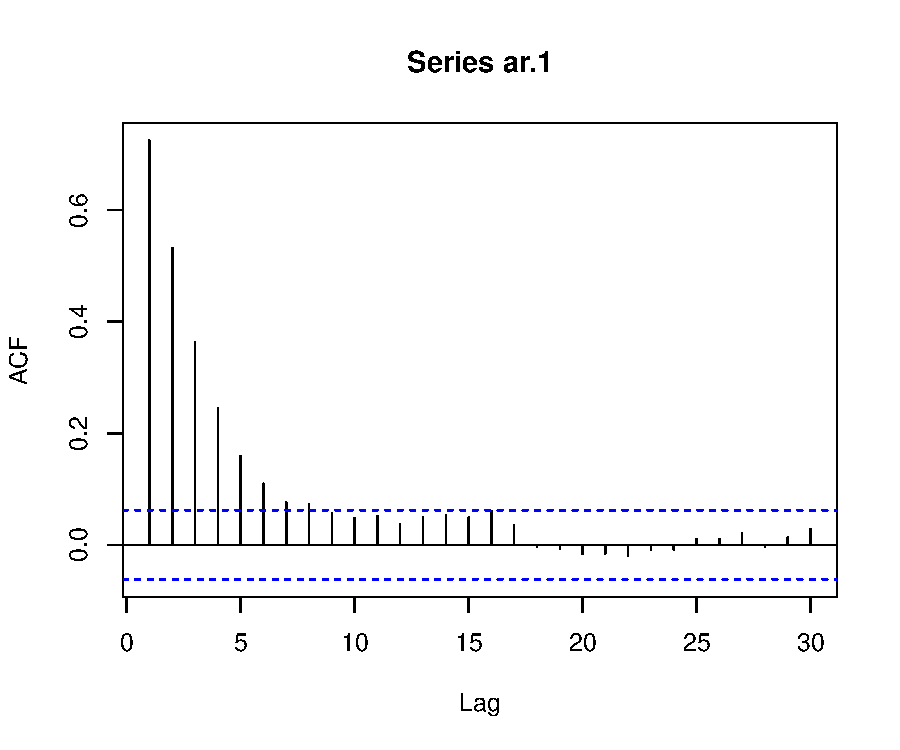
\includegraphics[width=0.47\linewidth]{images/ar1-acf-q6}}
    \caption{The AR(1) time series with $\boldsymbol{\phi=0.7}$}
    \label{ar1-q6}
\end{figure}
\begin{figure}[H]
    \centering
    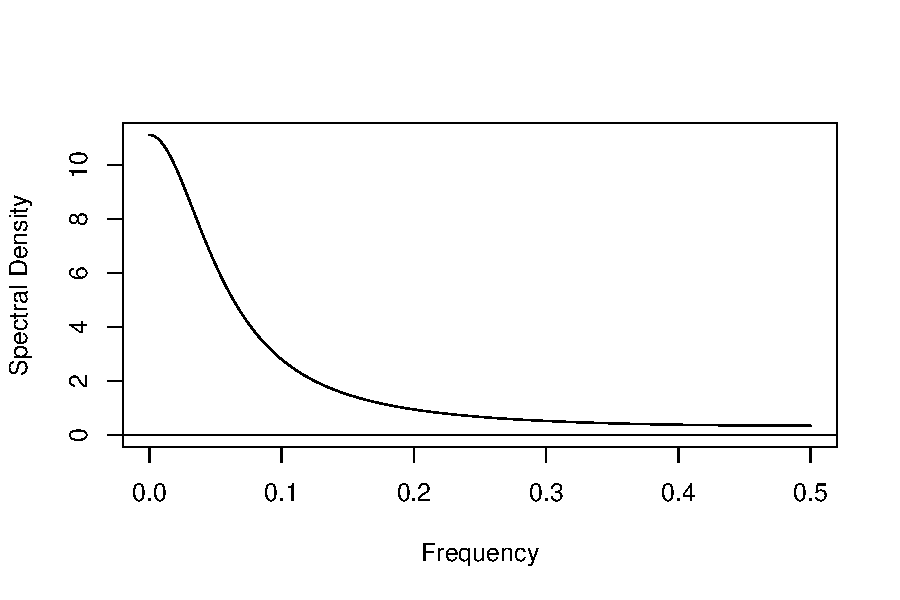
\includegraphics[width=0.65\linewidth]{images/ar1-spec}
    \caption{The theoretical spectral density of AR(1) time series with $\boldsymbol{\phi=0.7}$}
    \label{ar1-spec}
\end{figure}

\vspace{4pt}
\textbf{Subproblem (c)}

We plot the simulated $AR(1)$ time series with $\phi=-0.4$ as Figure \ref{ar1-q6-2}. As we can see 
from Figure \ref{ar1-q6-2}, because $\phi=-0.4$ is less than 0, so there is very strong variation in the time series. And we can see that 
the ACF is positive and negative alternate.


\vspace{4pt}

We graph the theoretical spectral density for an $AR(1)$ time series with $\phi=-0.4$ as Figure \ref{ar1-spec-2}. 
As we can see from Figure \ref{ar1-spec-2}, the spectral density is increasing with the increasing of frequency, which is agreed with 
the conclusion derived in subproblem (a). Besides, the density is much stonger for higher frequencies than for low frequencies, this is because the time series's variation is 
very strong, which means the process tends to oscillate back and forth across its mean level quickly.
\begin{figure}[H]
    \centering
    \subfigure[The AR(1) time series]{\label{}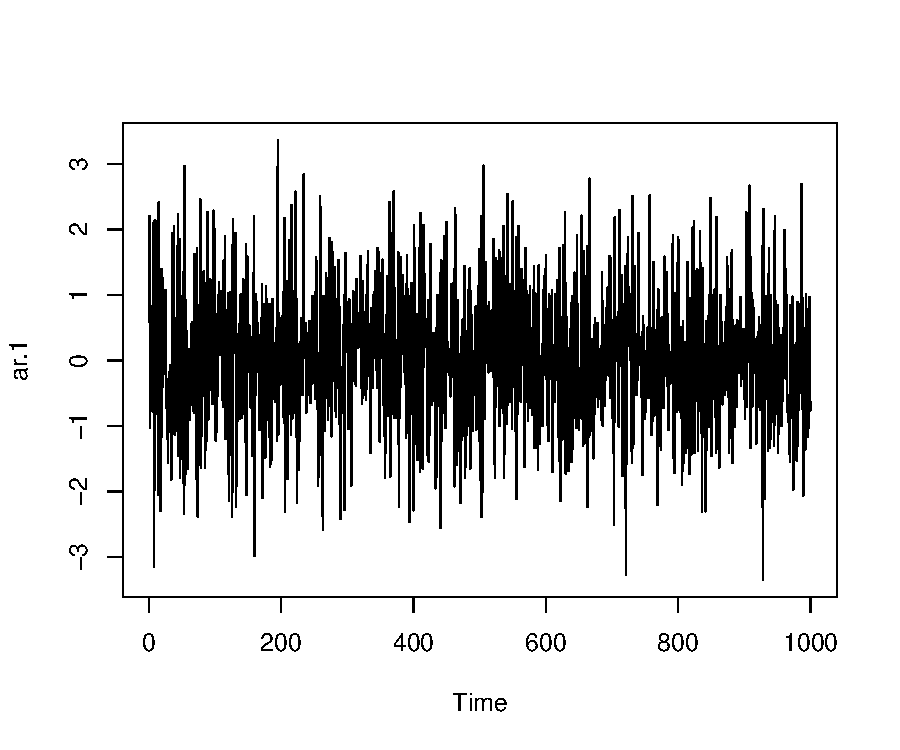
\includegraphics[width=0.47\linewidth]{images/ar1-q6-2}}
    \quad
    \subfigure[The acf of AR(1) time series]{\label{}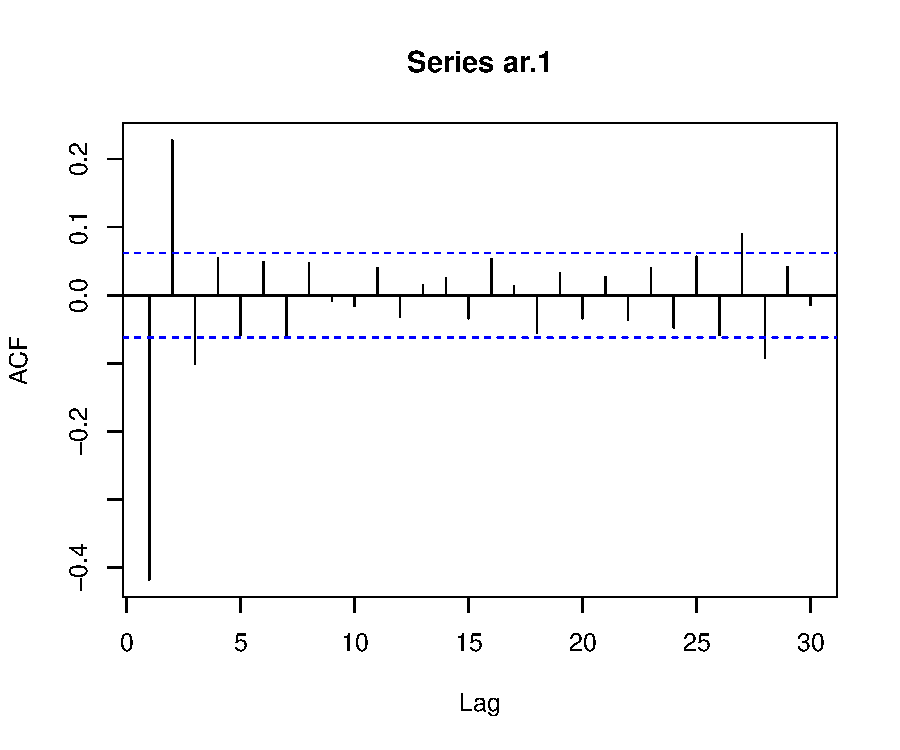
\includegraphics[width=0.47\linewidth]{images/ar1-acf-q6-2}}
    \caption{The AR(1) time series with $\boldsymbol{\phi=-0.4}$}
    \label{ar1-q6-2}
\end{figure}
\begin{figure}[H]
    \centering
    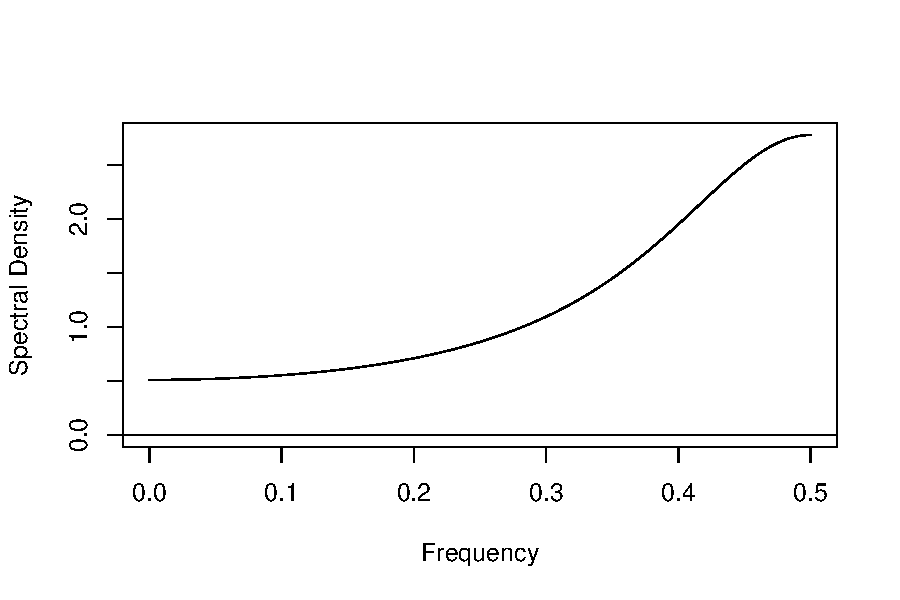
\includegraphics[width=0.65\linewidth]{images/ar1-spec-2}
    \caption{The theoretical spectral density of AR(1) time series with $\boldsymbol{\phi=-0.4}$}
    \label{ar1-spec-2}
\end{figure}

\end{homeworkProblem}

\begin{homeworkProblem}
Consider the $MA(1)$ model
$$
Y_{t}=e_{t}-\theta e_{t-1}
$$
The theoretical spectral density is:
$$
S(f)=\left[1+\theta^{2}-2 \theta \cos (2 \pi f)\right] \sigma_{e}^{2}
$$  
\begin{enumerate}[(a)]
    \item Graph the theoretical spectral density for an $M A(1)$ process with $\theta=0.6$. Interpret the implications of the shape of the spectrum on the possible plots of the time series values.
    \item Graph the theoretical spectral density for an $M A(1)$ process with $\theta=-0.8$. Interpret the implications of the shape of the spectrum on the possible plots of the time series values.
\end{enumerate}

\vspace{4pt}
\textbf{\large{Solution}}

\vspace{4pt}
\textbf{Subproblem (a)}

We plot the simulated $MA(1)$ time series with $\theta=0.6$ as Figure \ref{ma1--0.6}.

\vspace{4pt}
We graph the theoretical spectral density for an $MA(1)$ time series with $\theta=0.6$ as Figure \ref{ma1-spec--0.6}. 
As we can see from Figure \ref{ma1-spec--0.6}, the spectral density is increasing with the increasing of frequency. Besides, the density is much stonger for higher frequencies than for low frequencies, this is because the time series's variation is 
very strong, which means the process tends to oscillate back and forth across its mean level quickly.
\begin{figure}[H]
    \centering
    \subfigure[The AR(1) time series]{\label{}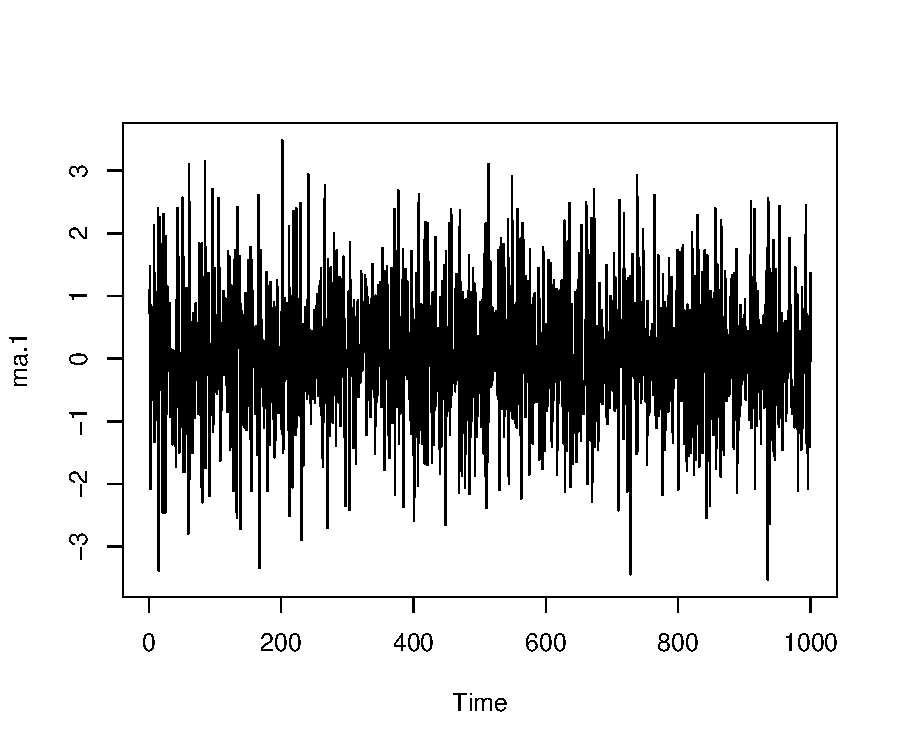
\includegraphics[width=0.47\linewidth]{images/ma1--0.6}}
    \quad
    \subfigure[The acf of AR(1) time series]{\label{}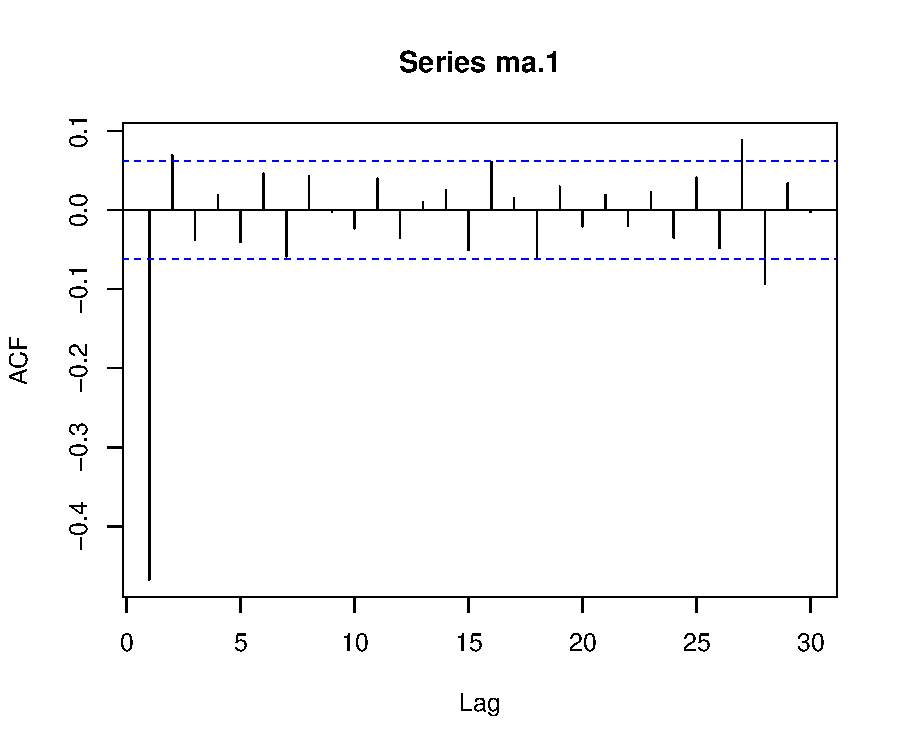
\includegraphics[width=0.47\linewidth]{images/ma1--0.6-acf}}
    \caption{The MA(1) time series with $\boldsymbol{\theta=0.6}$}
    \label{ma1--0.6}
\end{figure}
\begin{figure}[H]
    \centering
    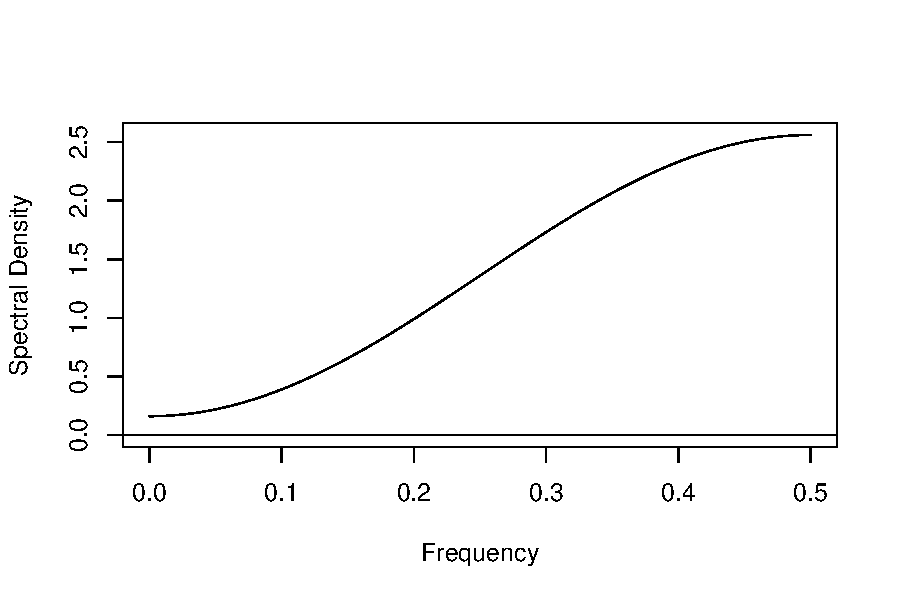
\includegraphics[width=0.65\linewidth]{images/ma1-spec--0.6}
    \caption{The theoretical spectral density of MA(1) time series with $\boldsymbol{\theta=0.6}$}
    \label{ma1-spec--0.6}
\end{figure}

\vspace{4pt}
\textbf{Subproblem (b)}

We plot the simulated $MA(1)$ time series with $\theta=-0.8$ as Figure \ref{ma1-0.8}. 

\vspace{4pt}
We graph the theoretical spectral density for an $MA(1)$ time series with $\theta=-0.8$ as Figure \ref{ma1-spec-0.8}. 
As we can see from Figure \ref{ma1-spec-0.8}, the spectral density is decreasing with the increasing of frequency. Besides, the density is much stonger for lower frequencies than for high frequencies, this is because the time series's variation is 
not very strong, which means the process tends to change slowly from one time instance to the next.
\begin{figure}[H]
    \centering
    \subfigure[The MA(1) time series]{\label{}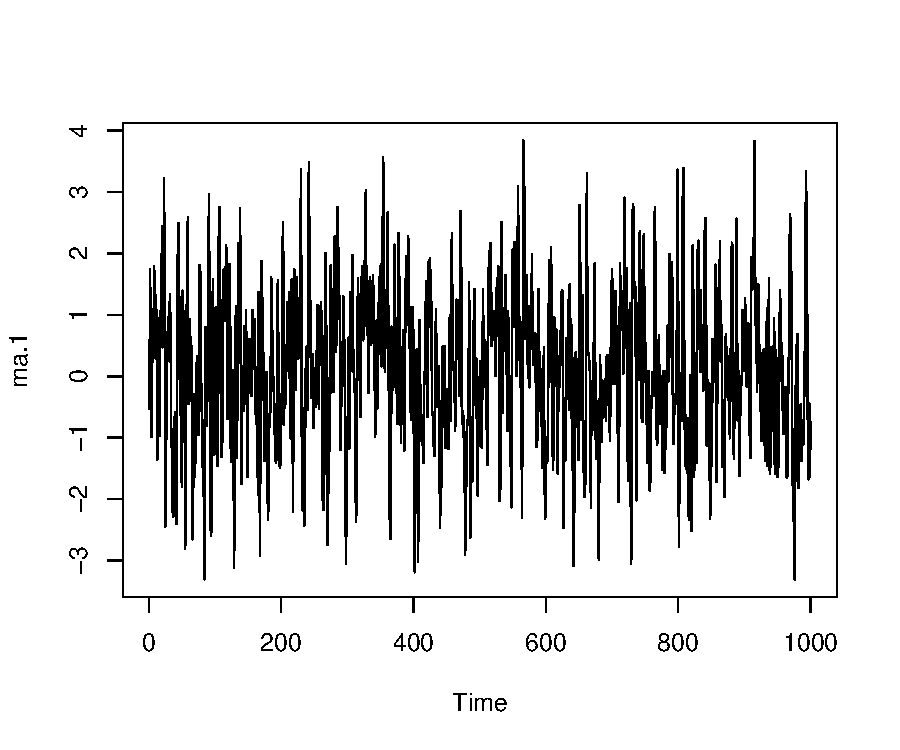
\includegraphics[width=0.47\linewidth]{images/ma1-0.8}}
    \quad
    \subfigure[The acf of MA(1) time series]{\label{}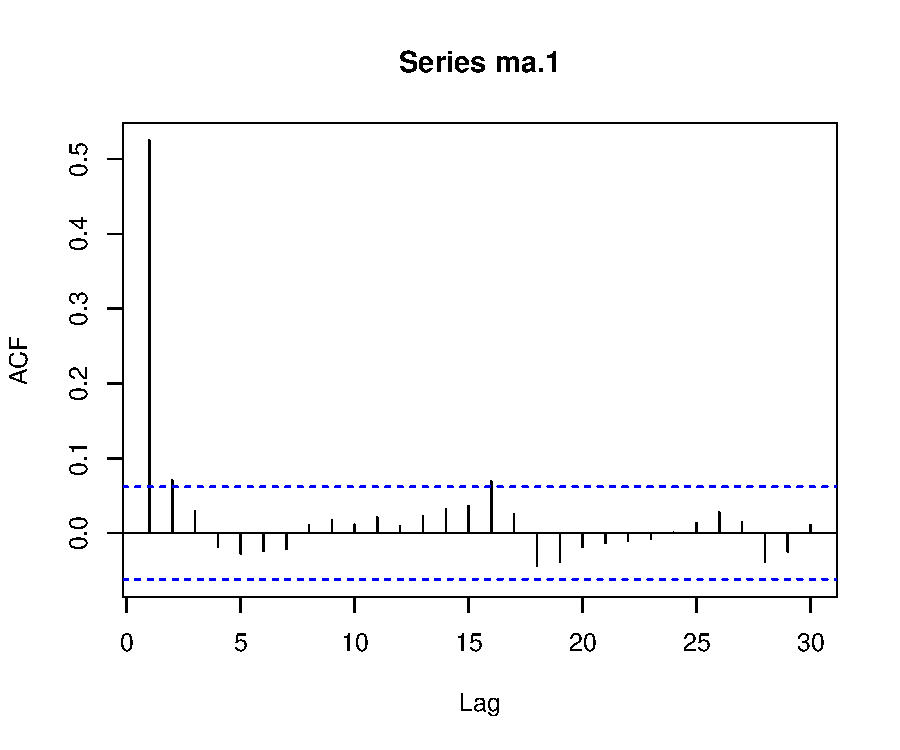
\includegraphics[width=0.47\linewidth]{images/ma1-0.8-acf}}
    \caption{The MA(1) time series with $\boldsymbol{\theta=-0.8}$}
    \label{ma1-0.8}
\end{figure}
\begin{figure}[H]
    \centering
    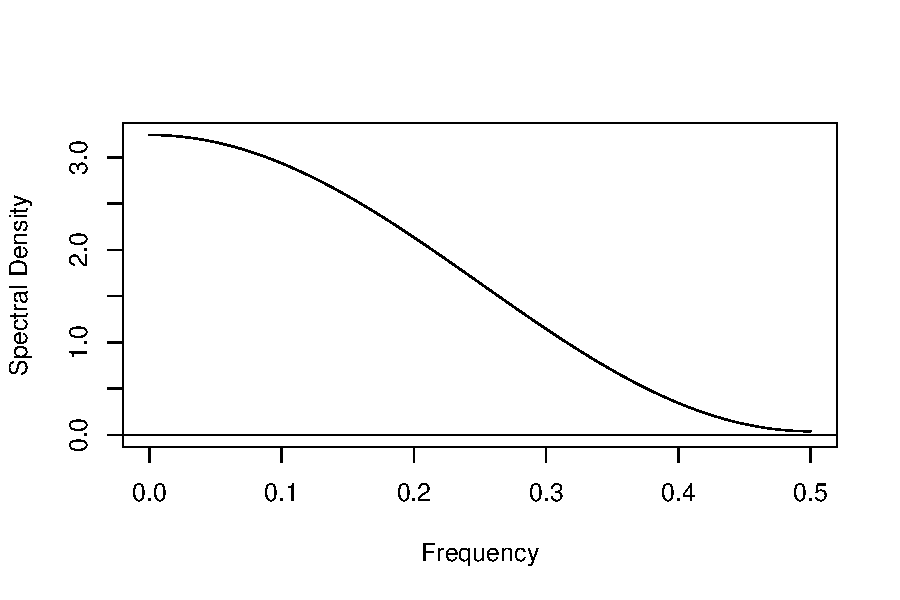
\includegraphics[width=0.65\linewidth]{images/ma1-spec-0.8}
    \caption{The theoretical spectral density of MA(1) time series with $\boldsymbol{\theta=-0.8}$}
    \label{ma1-spec-0.8}
\end{figure}
\end{homeworkProblem}

\end{document}

